\begin{ParaColumn}[\bisection*{Criteria of Static Liquefaction}{静态液化的判别标准}]
    
    In the conventional plasticity theory, instability is assumed to occur when the stress state reaches the failure surface. However, the occurrence of static liquefaction induces the unstable behavior of saturated soils before the failure stress state is reached \citep{Daouadji2010}, and the shear stress decreases after the onset of static liquefaction. The instability line often was used to judge the stable or unstable behavior of the soil, and it is obtained generally from experimental results. The instability condition of soil could be investigated theoretically on the basis of a second-order work criterion, which has been used to check the onset of instability or strain softening by \citet{Valanis1985} and \citet{Chu1992}. Whether the second-order work criterion is sufficient for instability or not has been studied \citep{Lade1987, Lade1988, Chu1993, Chu2009}. Here, the second-order work criterion was used to study the static liquefaction of sands with different initial void ratios under isotropically consolidated and K0-consolidated undrained triaxial condition, and the typical stress paths studied are shown in \enautoref{figure:2}.

    \switchcolumn

    在传统的塑性理论中,假定应力状态到达破坏面时会发生不稳定性。但是,静态液化的发生会在达到破坏应力状态之前引起饱和土的不稳定行为\citep{Daouadji2010},并且在静态液化开始后剪切应力会降低。通常使用不稳定性线来判断土壤的稳定或不稳定行为,通常可以从实验结果中获得。可以根据二阶功准则从理论上研究土体的失稳状况,该准则已由\citet{Valanis1985}和\citet{Chu1992}用于检查失稳或应变软化的发生。学者已经研究了二阶功准则是否足以满足不稳定要求\citep{Lade1987, Lade1988, Chu1993, Chu2009}。在这里,使用二阶功准则研究了在各向同性固结和$K_0$固结不排水的三轴条件下具有不同初始孔隙比的砂土的静态液化,所研究的典型应力路径如\cnautoref{figure:2}所示。

    \CrossColumnText{
        \begin{figure}[htb]
    \centering
    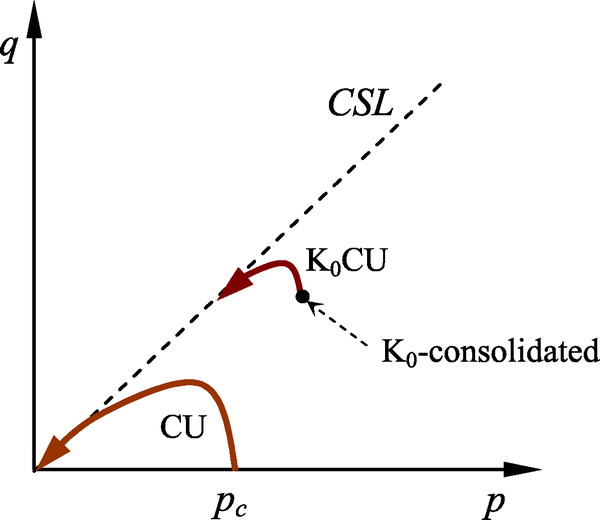
\includegraphics[width=.5\textwidth]{figures/figure2.jpg}
    \bicaption{Stress path analyzed (CU = consolidated undrained compression triaxial test; $K_{0}\mathrm{CU}=K_{0}$-consolidated undrained compression triaxial test; CSL = critical state line)}{应力路径分析(CU为固结不排水三轴试验; $K_{0}\mathrm{CU}$为$K_ {0}$固结不排水三轴试验; CSL为临界状态线)}
    \label{figure:2}
\end{figure}
    }
    \switchcolumn*

    in an infinitesimal deformation condition, according to the second-order work criterion, the stability of material requires

    \switchcolumn

    在无限小变形条件下,根据二阶功准则,材料的稳定性要求为

    \CrossColumnText{
        \begin{align}
            d^{2} w=d \widetilde{\sigma}^{\prime}: d \tilde{\varepsilon}>0, \quad \forall\|d \tilde{\varepsilon}\| \neq 0
            \label{equation:23}
        \end{align}
    }
    \switchcolumn*

    \noindent
    where $d^{2} w$ = second-order work; $d \widetilde{\sigma}^{\prime}$ = effective stress increment; and $d \tilde{\varepsilon}$ = corresponding strain increment.

    \switchcolumn

    \noindent
    式中,$d^{2} w$为二阶功,$d \widetilde{\sigma}^{\prime}$为有效应力增量,$d \tilde{\varepsilon}$为对应的应变增量。

    \switchcolumn*

    It could be inferred that, if there exists a loading path that results in the violation of \enautoref{equation:23}, the material becomes potentially unstable, so the condition of the potential instability is

    \switchcolumn

    可以推断出,如果存在导致违反\cnautoref{equation:23}的加载路径,则材料可能会变得不稳定,因此潜在的不稳定条件为

    \CrossColumnText{
        \begin{align}
            d^{2} w=d \widetilde{\sigma}^{\prime}: d \tilde{\varepsilon} \leq 0, \quad \exists\|d \tilde{\varepsilon}\| \neq 0
            \label{equation:24}
        \end{align}
    }

    \switchcolumn*

    \noindent
    After inserting \enautoref{equation:11} or \enautoref{equation:20}, one gets

    \switchcolumn

    \noindent
    将\cnautoref{equation:11}代入\cnautoref{equation:20},得到

    \CrossColumnText{
        \begin{align}
            d \tilde{\varepsilon}: \mathbf{D}^{e p}: d \tilde{\varepsilon} \leq 0, \quad \exists\|d \tilde{\varepsilon}\| \neq 0
            \label{equation:25}
        \end{align}
    }
    \switchcolumn*

    \noindent
    \enautoref{equation:25}implies the vanishing determinant value of the symmetric part

    \switchcolumn

    \noindent
    \cnautoref{equation:25}隐含着对称部分的行列式值

    \CrossColumnText{
        \begin{align}
            \operatorname{det}\left(\mathbf{D}_{\mathrm{sys}}^{e p}\right) \leq 0
            \label{equation:26}
        \end{align}
    }
    \switchcolumn*

    \noindent
    When under a triaxial condition, the criterion of \enautoref{equation:26} becomes

    \switchcolumn

    \noindent
    在三轴条件下,\cnautoref{equation:26}变为

    \CrossColumnText{
        \begin{align}
            \operatorname{det}\left[\left(\mathbf{D}_{p q}^{e p}\right)_{\mathrm{sys}}\right] \leq 0
            \label{equation:27}
        \end{align}
    }
    \switchcolumn*

    \enautoref{equation:24} also could be expressed by replacing the strain increment with stress rate

    \switchcolumn

    \cnautoref{equation:24}也可以通过用应力率代替应变增量来表示

    \CrossColumnText{
        \begin{align}
            d \widetilde{\boldsymbol{\sigma}}^{\prime}: \mathbf{C}^{e p}: d \widetilde{\boldsymbol{\sigma}}^{\prime} \leq 0, \quad \exists\left\|d \widetilde{\boldsymbol{\sigma}}^{\prime}\right\| \neq 0
        \end{align}
    }
    \switchcolumn*

    \noindent
    where $\mathbf{C}^{e p}$ = inversion of $\mathbf{D}^{e p}$. The determinant of the symmetric part of both tensors goes to zero simultaneously \citep{Prunier2009}, so the analysis based on both tensors would give the same results.

    \switchcolumn

    \noindent
    其中$\mathbf{C}^{e p}$为$\mathbf{D}^{e p}$的逆矩阵。 两个张量的对称部分的行列式同时变为零\citep{Prunier2009},因此基于两个张量的分析将得出相同的结果。

    \switchcolumn*

    It should be noted that Eqs. \ref{equation:26} and \ref{equation:27} are necessary but insufficient conditions of \enautoref{equation:25}. Once \enautoref{equation:26} is satisfied, the soil becomes potentially unstable and the stability depends on the stress increment. It could be inferred that the soil could stay stable as long as the stress increment is not along the unstable stress path, even if the soil is potentially unstable. Also, it should be noted that the negative value of the second-order work is necessary but insufficient for the static liquefaction \citep{Chu2001}, and the additional conditions are \citep{Lade1992}

    \switchcolumn

    应该注意的是,\cnautoref{equation:26}和\cnautoref{equation:27}是必要的,但\cnautoref{equation:25}的条件不足。 一旦\cnautoref{equation:26}满足,土体变得潜在不稳定,稳定性取决于应力增量。 可以推断,即使应力增加不沿着不稳定的应力路径,土体也可以保持稳定,即使土体可能是不稳定的。 另外,应该指出的是,二阶功的负值是必要的,但对于静态液化来说是不足的\citep{Chu2001},附加条件是\citep{Lade1992}。

    \CrossColumnText{
        \begin{align}
            \begin{array}{l}
            \frac{\partial F}{\partial \sigma_{i j}} \cdot \delta_{i j}<0 \\
            \frac{\partial Q}{\partial \sigma_{i j}} \cdot \delta_{i j}>0
            \end{array}
            \label{equation:29}
        \end{align}
    }
    \switchcolumn*

    \noindent
    By substituting Eqs. \ref{equation:3} and \ref{equation:8} into \enautoref{equation:29}, the first inequality is satisfied, and the second inequality requires $M_d-M>0$. It can be concluded that the tendency of volumetric compression of the soil under undrained conditions combined with the violation of second-order work yield the complete condition for static liquefaction to occur.

    \switchcolumn

    \noindent
    通过将\cnautoref{equation:3}和\cnautoref{equation:8}代入\cnautoref{equation:29},第一个不等式得到满足,第二个不等式要求$M_d-M>0$。 可以得出结论,在不排水的条件下土体的体积压缩趋势加上违反二阶功的情况为静态液化发生提供了完整条件。

\end{ParaColumn}